%%
%% Author: thompson
%% 03.11.17
%%

% Preamble
\documentclass[11pt]{article}

% Packages
\usepackage{a4wide}
\usepackage[ngerman]{babel}
\usepackage[utf8]{inputenc}

\usepackage{scrextend}
\usepackage{enumerate}
\usepackage{graphicx}
\usepackage{verbatim}

% Document
\begin{document}
    \section{Analysis mit Wireshark}
    Im Rahmen dieser Sektion wollen wir eine weitere Datei analysieren, welche mit Wireshark aufgenommen wurde, dump\_http.pcap.
    \begin{enumerate}[\thesection .1]
        \item Welche Objekte wurden vom Klienten via HTTP angefordert?
        Mithilfe von
        \begin{verbatim}
            File > Export Objects > HTTP...
        \end{verbatim}
        kann man direkt einsehen, welche Elemente im Rahmen aller HTTP-Protokollierten Frames, innerhalb des derzeitig geladenen .pcap übertragen wurden.
        In unserem dump\_http.pcap wurden die Elemente text(145 Byte, Frame 6), logo.gif(4445 Byte, Frame 22) und TechnikErleben.png(27 kB, Frame 66) angefordert, von 192.168.1.10.
        \item Recherchieren Sie die Bedeutung der einzelnen Header-Felder bei den Anfragen bzw. Antworten des Servers.
        TCP-Header bestimmen eine ganze Reihe an diversen Datensätzen. Über 10 Felder von je 20 bytes \& zusätzlichen 40 byte
        an optionalen, informativen Daten, bestimmt man\\\\

        $\diamond$ Sender TCP Port Nummer (2 Byte)
        \begin{addmargin}[1em]{1em}
            Der spezifizierte Port, von welchem der Sender sendet.
        \end{addmargin}

        $\diamond$ Empfänger TCP Port Nummer (2 Byte)
        \begin{addmargin}[1em]{1em}
            Der spezifizierte Port, wo der Empfänger die Nachricht erhält.
        \end{addmargin}

        $\diamond$ Sequenznummer (4 Byte)
        \begin{addmargin}[1em]{1em}
            ... sie dient der Information über die Menge bereits gesendeter Data. Sie ist in jedem Datenpacket vorhanden und
            dient mitsamt der Acknowledge Nummer (next §) dazu, dem Sender den erfolgreichen Transfer zu übermitteln. Zwecks Sicherheitsvorkehrungen startet diese immer
            mit einem zufälligen Wert zwischen 0 und $(2^32)-1$. Wireshark bietet hinsichtlich der X-hunderten Zahlenwerten eine relative
            Sequenznummer an, um die Packetidentifikation in mehreren Hinsichten zu vereinfachen.\\\\
            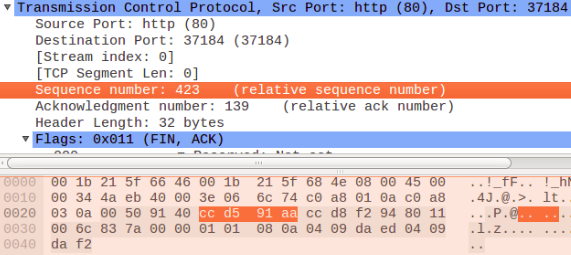
\includegraphics[width=30em, height=15em]{SequenceNumber.png}
        \end{addmargin}
\pagebreak
        $\diamond$ Acknowledge number (4 Byte)
        \begin{addmargin}[1em]{1em}
            Diese dient dazu den Datentransfer zu bestätigen.
            Prinzipiell gilt, dass die geantwortete ACK zur neuen SEQ wird, siehe auch
            \begin{center}
                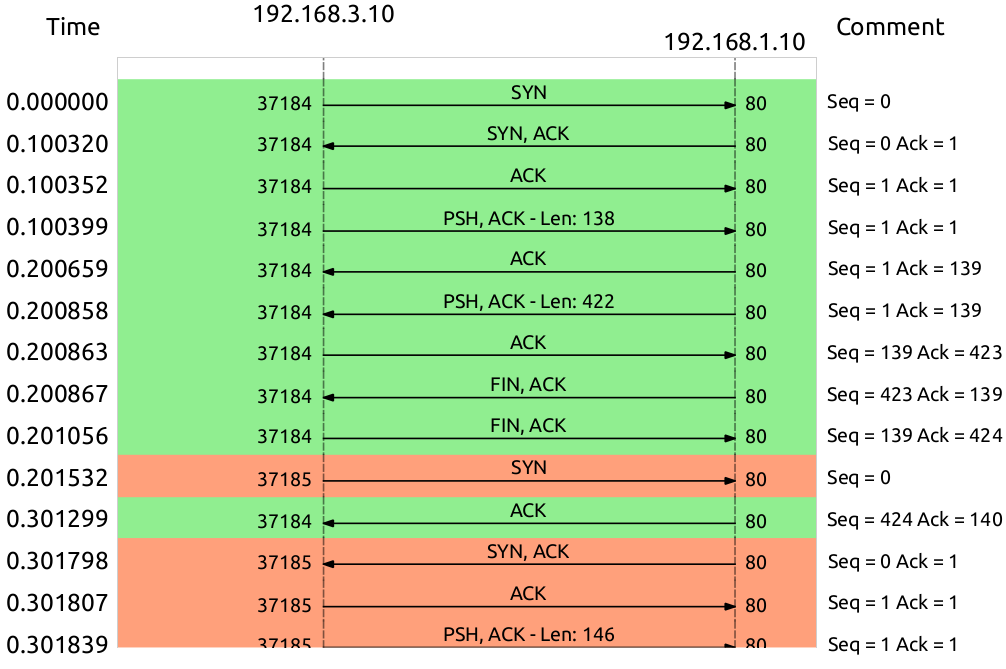
\includegraphics[width=\textwidth]{SeqAckFlowgraph.png}
            \end{center}

            ... Via Wireshark, lässt sich ein solcher Graph mittels
            \begin{verbatim}
                Statistics > Flow Graph > Flow Type: TCP flow
            \end{verbatim}
            erstellen.

        \end{addmargin}

        $\diamond$ TCP Data Offset (X words ... 8 Bytes each)
        \begin{addmargin}[1em]{1em}
            .. dieser dient zur Spezifikation des eigentlichen Dateistarts.
            Anhand von 'Header Length: xx Byte' lässt sich dies feststellen.
        \end{addmargin}

        $\diamond$ Reserved Data (4 Bit)
        \begin{addmargin}[1em]{1em}
            Das Reserved Data-Feld ist für zukünftige Verwendungen reserviert. Alle Bits müssen null sein.
            % // FIXME: Didn't find this sucker in Wireshark. Repair it.
        \end{addmargin}

        $\diamond$ Control Flags (8 Bit)
        \begin{addmargin}[1em]{1em}
            Beschrieben durch 2 Variablen oder 4 Hexa-Werten.
            Zu den möglichen Flags gehören:
            \begin{itemize}
                \item ECE - Explicit Congestion Notification (ECN-ECHO): Bei Netzwerküberlastung
                \item CWR - Congestion Window Reduced: Revertiert ECE
                \item URG - Urgent: Selten genutzt, oftmals als Interrupt-Signal
                \item ACK - Acknowledgement: Setzt Gültigkeit für Sequenz/Acknowledge-Values
                \item PSH - Push: Umgehung lokaler Puffer für schnellere Übertragung
                \item RST - Reset: Zum Abbruch von Verbindungen
                \item SYN - Initiieren der Verbindung. Üblicherweise beantwortet mit SYN+ACK oder RST
                \item FIN - Finish: Schlussflag, dient zur Freigabe der Verbindung \& Bestätigt vollständige Übertragung.\\
            \end{itemize}
            \begin{center}
                Bezüglich PSH: Datenverkehr \& Pufferfunktion bei Übertragung
                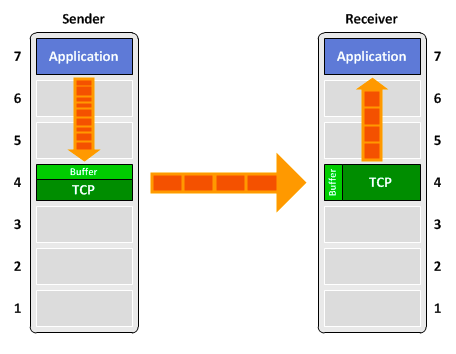
\includegraphics[width=0.7\textwidth]{PSHAndBuffer.png}
            \end{center}
        \end{addmargin}

        $\diamond$ Window size (2 Bytes)
        \begin{addmargin}[1em]{1em}
            Bestimmt die Puffergröße bezüglich der zu sendenden Daten.
            Dies steht in Relation mit ACK, da der Datensatz erst mit der ACK-Nummer bestätigt wird.
            e.g.: Bei zu klein gewähltem Puffer muss der Sender eines Elementes auf die Antwort des Empfängers warten, bevor
            dieser weitere Packete des jeweiligen Elementes senden darf.
        \end{addmargin}

        $\diamond$ TCP checksum (2 Byte)
        \begin{addmargin}[1em]{1em}
            Die Prüfsumme des TCP-Headers dient der Erkennung von Fehlübertragungen, bestehend aus Empfänger-IP,
            Sender-IP, TCP-Protokollerkennung, Länge des TCP-Headers und Nutzdaten.

        \end{addmargin}

        \item Wie viele TCP-Verbindungen werden insgesamt aufgebaut? Wie unterscheidet sich das von dump\_protocols.pcap?
        Mithilfe des Filters \textbf{'tcp \&\& !http'} können wir insgesamt 68 TCP-Frames feststellen.
        \item Bestimmen Sie, wie viele Bytes in jeder Verbindung ausgetauscht werden und wie lange die einzelnen Verbindungen bestehen.
    \end{enumerate}

\end{document}